\documentclass[tikz,border=4pt]{standalone}
\usepackage{amsmath,amssymb}

\usetikzlibrary{arrows.meta,positioning,automata,shapes,shapes.misc,calc,decorations.pathmorphing,decorations.markings,angles,quotes,patterns,mindmap,matrix,knots,hobby,trees}
\tikzset{->-/.style={decoration={markings, mark=at position 0.5 with {\arrow{Stealth}}}, postaction={decorate}}}
\begin{document}
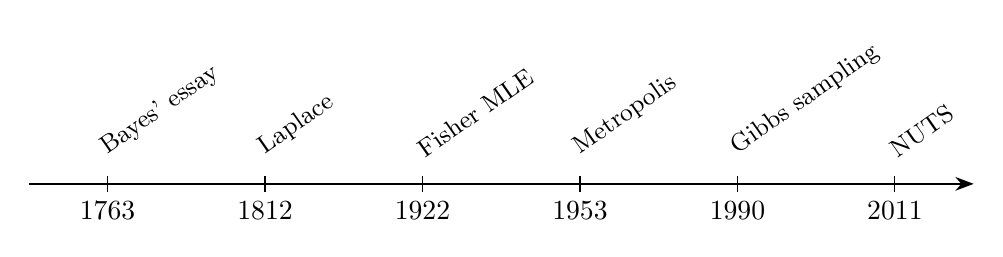
\begin{tikzpicture}[>=Stealth]
\draw[->, thick] (0,0) -- (12,0);
\foreach \x/\y/\l in {1/1763/Bayes' essay, 3/1812/Laplace, 5/1922/Fisher MLE, 7/1953/Metropolis, 9/1990/Gibbs sampling, 11/2011/NUTS} {
  \draw (\x,0.1) -- (\x,-0.1) node[below] {\y};
  \node[above, rotate=35, anchor=south west, font=\small] at (\x,0.15) {\l};
}
\end{tikzpicture}
\end{document}
